\documentclass{standalone}
\usepackage{tikz}
\usetikzlibrary{patterns, positioning}


\begin{document}
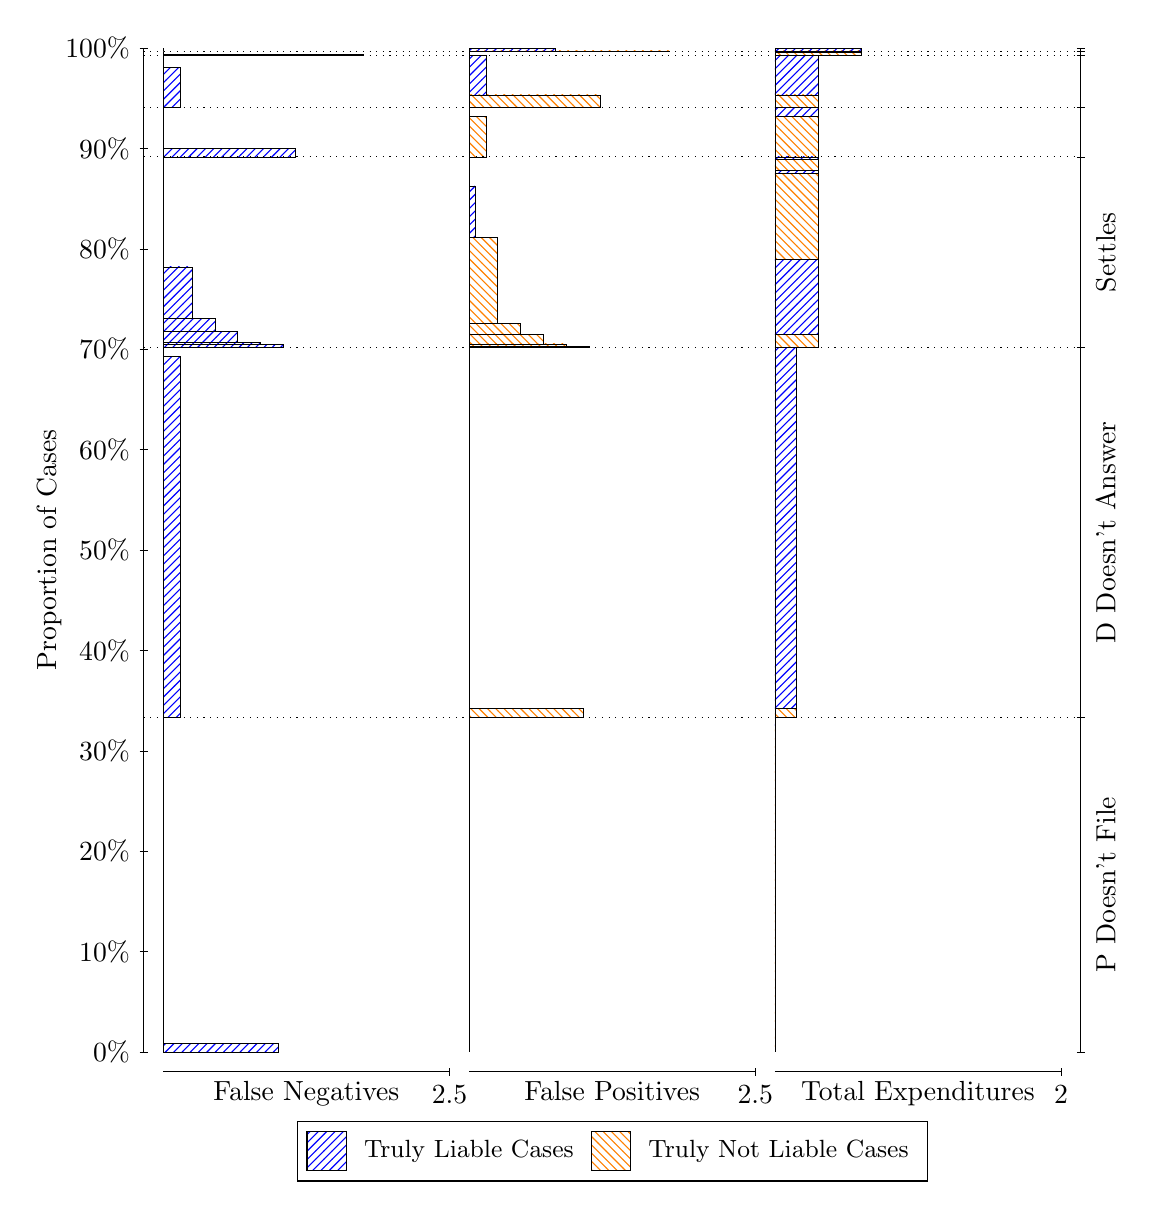
\begin{tikzpicture}
\draw[black, very thin] (1.5,1.75) -- (1.5,14.5);
\node[rotate=90, text=black, anchor=center] at (0.3, 8.125) {Proportion of Cases};
\draw[black, very thin] (1.45,1.75) -- (1.55,1.75);
\node[text=black, anchor=east] at (1.45, 1.75) {0\%};
\draw[black, very thin] (1.45,3.025) -- (1.55,3.025);
\node[text=black, anchor=east] at (1.45, 3.025) {10\%};
\draw[black, very thin] (1.45,4.3) -- (1.55,4.3);
\node[text=black, anchor=east] at (1.45, 4.3) {20\%};
\draw[black, very thin] (1.45,5.575) -- (1.55,5.575);
\node[text=black, anchor=east] at (1.45, 5.575) {30\%};
\draw[black, very thin] (1.45,6.85) -- (1.55,6.85);
\node[text=black, anchor=east] at (1.45, 6.85) {40\%};
\draw[black, very thin] (1.45,8.125) -- (1.55,8.125);
\node[text=black, anchor=east] at (1.45, 8.125) {50\%};
\draw[black, very thin] (1.45,9.4) -- (1.55,9.4);
\node[text=black, anchor=east] at (1.45, 9.4) {60\%};
\draw[black, very thin] (1.45,10.675) -- (1.55,10.675);
\node[text=black, anchor=east] at (1.45, 10.675) {70\%};
\draw[black, very thin] (1.45,11.95) -- (1.55,11.95);
\node[text=black, anchor=east] at (1.45, 11.95) {80\%};
\draw[black, very thin] (1.45,13.225) -- (1.55,13.225);
\node[text=black, anchor=east] at (1.45, 13.225) {90\%};
\draw[black, very thin] (1.45,14.5) -- (1.55,14.5);
\node[text=black, anchor=east] at (1.45, 14.5) {100\%};

\draw[black, very thin] (13.4,1.75) -- (13.4,14.5);
\draw[black, very thin] (13.35,1.75) -- (13.45,1.75);
\node[anchor=west] at (13.35, 1.75) {};
\draw[black, very thin] (13.35,5.9956) -- (13.45,5.9956);
\node[anchor=west] at (13.35, 5.9956) {};
\draw[black, very thin] (13.35,10.7) -- (13.45,10.7);
\node[anchor=west] at (13.35, 10.7) {};
\draw[black, very thin] (13.35,13.117) -- (13.45,13.117);
\node[anchor=west] at (13.35, 13.117) {};
\draw[black, very thin] (13.35,13.746) -- (13.45,13.746);
\node[anchor=west] at (13.35, 13.746) {};
\draw[black, very thin] (13.35,14.409) -- (13.45,14.409);
\node[anchor=west] at (13.35, 14.409) {};
\draw[black, very thin] (13.35,14.457) -- (13.45,14.457);
\node[anchor=west] at (13.35, 14.457) {};
\draw[black, very thin] (13.35,14.5) -- (13.45,14.5);
\node[anchor=west] at (13.35, 14.5) {};

\draw[black, very thin, pattern color=blue, pattern=north east lines] (1.75,1.75) rectangle (3.2033,1.8582);
\draw[black, very thin, pattern color=orange, pattern=north west lines] (1.75,1.8582) rectangle (1.75,5.9956);
\draw[black, very thin, pattern color=blue, pattern=north east lines] (1.75,5.9956) rectangle (1.968,10.584);
\draw[black, very thin, pattern color=orange, pattern=north west lines] (1.75,10.584) rectangle (1.75,10.7);
\draw[black, very thin, pattern color=blue, pattern=north east lines] (1.75,10.7) rectangle (3.276,10.733);
\draw[black, very thin, pattern color=blue, pattern=north east lines] (1.75,10.733) rectangle (2.9853,10.766);
\draw[black, very thin, pattern color=blue, pattern=north east lines] (1.75,10.766) rectangle (2.6947,10.899);
\draw[black, very thin, pattern color=blue, pattern=north east lines] (1.75,10.899) rectangle (2.404,11.068);
\draw[black, very thin, pattern color=blue, pattern=north east lines] (1.75,11.068) rectangle (2.1133,11.721);
\draw[black, very thin, pattern color=orange, pattern=north west lines] (1.75,11.721) rectangle (1.75,13.117);
\draw[black, very thin, pattern color=blue, pattern=north east lines] (1.75,13.117) rectangle (3.4213,13.229);
\draw[black, very thin, pattern color=orange, pattern=north west lines] (1.75,13.229) rectangle (1.75,13.746);
\draw[black, very thin, pattern color=blue, pattern=north east lines] (1.75,13.746) rectangle (1.968,14.25);
\draw[black, very thin, pattern color=orange, pattern=north west lines] (1.75,14.25) rectangle (1.75,14.409);
\draw[black, very thin, pattern color=blue, pattern=north east lines] (1.75,14.409) rectangle (4.2933,14.416);
\draw[black, very thin, pattern color=orange, pattern=north west lines] (1.75,14.416) rectangle (1.75,14.457);
\draw[black, very thin, pattern color=orange, pattern=north west lines] (1.75,14.457) rectangle (1.75,14.465);
\draw[black, very thin, pattern color=blue, pattern=north east lines] (1.75,14.465) rectangle (1.75,14.5);
\draw[black, very thin, pattern color=orange, pattern=north west lines] (5.6333,1.75) rectangle (5.6333,5.8874);
\draw[black, very thin, pattern color=blue, pattern=north east lines] (5.6333,5.8874) rectangle (5.6333,5.9956);
\draw[black, very thin, pattern color=orange, pattern=north west lines] (5.6333,5.9956) rectangle (7.0867,6.1119);
\draw[black, very thin, pattern color=blue, pattern=north east lines] (5.6333,6.1119) rectangle (5.6333,10.7);
\draw[black, very thin, pattern color=orange, pattern=north west lines] (5.6333,10.7) rectangle (7.1593,10.71);
\draw[black, very thin, pattern color=orange, pattern=north west lines] (5.6333,10.71) rectangle (6.8687,10.743);
\draw[black, very thin, pattern color=orange, pattern=north west lines] (5.6333,10.743) rectangle (6.578,10.865);
\draw[black, very thin, pattern color=orange, pattern=north west lines] (5.6333,10.865) rectangle (6.2873,11.004);
\draw[black, very thin, pattern color=orange, pattern=north west lines] (5.6333,11.004) rectangle (5.9967,12.096);
\draw[black, very thin, pattern color=blue, pattern=north east lines] (5.6333,12.096) rectangle (5.706,12.748);
\draw[black, very thin, pattern color=blue, pattern=north east lines] (5.6333,12.748) rectangle (5.6333,13.117);
\draw[black, very thin, pattern color=orange, pattern=north west lines] (5.6333,13.117) rectangle (5.8513,13.634);
\draw[black, very thin, pattern color=blue, pattern=north east lines] (5.6333,13.634) rectangle (5.6333,13.746);
\draw[black, very thin, pattern color=orange, pattern=north west lines] (5.6333,13.746) rectangle (7.3047,13.906);
\draw[black, very thin, pattern color=blue, pattern=north east lines] (5.6333,13.906) rectangle (5.8513,14.409);
\draw[black, very thin, pattern color=orange, pattern=north west lines] (5.6333,14.409) rectangle (5.6333,14.451);
\draw[black, very thin, pattern color=blue, pattern=north east lines] (5.6333,14.451) rectangle (5.6333,14.457);
\draw[black, very thin, pattern color=orange, pattern=north west lines] (5.6333,14.457) rectangle (8.1767,14.465);
\draw[black, very thin, pattern color=blue, pattern=north east lines] (5.6333,14.465) rectangle (6.7233,14.5);
\draw[black, very thin, pattern color=orange, pattern=north west lines] (9.5167,1.75) rectangle (9.5167,5.8874);
\draw[black, very thin, pattern color=blue, pattern=north east lines] (9.5167,5.8874) rectangle (9.5167,5.9956);
\draw[black, very thin, pattern color=orange, pattern=north west lines] (9.5167,5.9956) rectangle (9.7892,6.1119);
\draw[black, very thin, pattern color=blue, pattern=north east lines] (9.5167,6.1119) rectangle (9.7892,10.7);
\draw[black, very thin, pattern color=orange, pattern=north west lines] (9.5167,10.7) rectangle (10.062,10.865);
\draw[black, very thin, pattern color=blue, pattern=north east lines] (9.5167,10.865) rectangle (10.062,11.82);
\draw[black, very thin, pattern color=orange, pattern=north west lines] (9.5167,11.82) rectangle (10.062,12.912);
\draw[black, very thin, pattern color=blue, pattern=north east lines] (9.5167,12.912) rectangle (10.062,12.945);
\draw[black, very thin, pattern color=orange, pattern=north west lines] (9.5167,12.945) rectangle (10.062,13.084);
\draw[black, very thin, pattern color=blue, pattern=north east lines] (9.5167,13.084) rectangle (10.062,13.117);
\draw[black, very thin, pattern color=orange, pattern=north west lines] (9.5167,13.117) rectangle (10.062,13.634);
\draw[black, very thin, pattern color=blue, pattern=north east lines] (9.5167,13.634) rectangle (10.062,13.746);
\draw[black, very thin, pattern color=orange, pattern=north west lines] (9.5167,13.746) rectangle (10.062,13.906);
\draw[black, very thin, pattern color=blue, pattern=north east lines] (9.5167,13.906) rectangle (10.062,14.409);
\draw[black, very thin, pattern color=orange, pattern=north west lines] (9.5167,14.409) rectangle (10.607,14.451);
\draw[black, very thin, pattern color=blue, pattern=north east lines] (9.5167,14.451) rectangle (10.607,14.457);
\draw[black, very thin, pattern color=orange, pattern=north west lines] (9.5167,14.457) rectangle (10.607,14.465);
\draw[black, very thin, pattern color=blue, pattern=north east lines] (9.5167,14.465) rectangle (10.607,14.5);
\draw[black, dotted] (1.5,5.9956) -- (13.4,5.9956);
\draw[black, dotted] (1.5,10.7) -- (13.4,10.7);
\draw[black, dotted] (1.5,13.117) -- (13.4,13.117);
\draw[black, dotted] (1.5,13.746) -- (13.4,13.746);
\draw[black, dotted] (1.5,14.409) -- (13.4,14.409);
\draw[black, dotted] (1.5,14.457) -- (13.4,14.457);
\draw[black, very thin] (1.75,1.5) -- (5.3833,1.5);
\node[text=black, anchor=north] at (3.5667, 1.5) {False Negatives};
\draw[black, very thin] (5.3833,1.45) -- (5.3833,1.55);
\node[text=black, anchor=north] at (5.3833, 1.45) {2.5};

\draw[black, very thin] (5.6333,1.5) -- (9.2667,1.5);
\node[text=black, anchor=north] at (7.45, 1.5) {False Positives};
\draw[black, very thin] (9.2667,1.45) -- (9.2667,1.55);
\node[text=black, anchor=north] at (9.2667, 1.45) {2.5};

\draw[black, very thin] (9.5167,1.5) -- (13.15,1.5);
\node[text=black, anchor=north] at (11.333, 1.5) {Total Expenditures};
\draw[black, very thin] (13.15,1.45) -- (13.15,1.55);
\node[text=black, anchor=north] at (13.15, 1.45) {2};

\node[text=black, centered, rotate=90] at (13.72, 3.8728) {P Doesn't File};
\node[text=black, centered, rotate=90] at (13.72, 8.3477) {D Doesn't Answer};
\node[text=black, centered, rotate=90] at (13.72, 11.908) {Settles};





\draw (7.449999999999999,1.5) node[draw=none] (baseCoordinate) {};
\begin{scope}[align=center]
        \matrix[scale=0.5, draw=black, below=0.5cm of baseCoordinate, nodes={draw}, column sep=0.1cm]{
            \node[rectangle, draw, minimum width=0.5cm, minimum height=0.5cm, pattern color=blue, pattern=north east lines] {}; &
            \node[draw=none, font=\small, text=black] (B) {Truly Liable Cases}; &
            \node[rectangle, draw, minimum width=0.5cm, minimum height=0.5cm, pattern color=orange, pattern=north west lines] {}; &
            \node[draw=none, font=\small, text=black] (B) {Truly Not Liable Cases}; \\
            };
\end{scope}

\end{tikzpicture}
\end{document}